\documentclass[twoside]{book}

% Packages required by doxygen
\usepackage{fixltx2e}
\usepackage{calc}
\usepackage{doxygen}
\usepackage{graphicx}
\usepackage[utf8]{inputenc}
\usepackage{makeidx}
\usepackage{multicol}
\usepackage{multirow}
\PassOptionsToPackage{warn}{textcomp}
\usepackage{textcomp}
\usepackage[nointegrals]{wasysym}
\usepackage[table]{xcolor}

% Font selection
\usepackage[T1]{fontenc}
\usepackage{mathptmx}
\usepackage[scaled=.90]{helvet}
\usepackage{courier}
\usepackage{amssymb}
\usepackage{sectsty}
\renewcommand{\familydefault}{\sfdefault}
\allsectionsfont{%
  \fontseries{bc}\selectfont%
  \color{darkgray}%
}
\renewcommand{\DoxyLabelFont}{%
  \fontseries{bc}\selectfont%
  \color{darkgray}%
}
\newcommand{\+}{\discretionary{\mbox{\scriptsize$\hookleftarrow$}}{}{}}

% Page & text layout
\usepackage{geometry}
\geometry{%
  a4paper,%
  top=2.5cm,%
  bottom=2.5cm,%
  left=2.5cm,%
  right=2.5cm%
}
\tolerance=750
\hfuzz=15pt
\hbadness=750
\setlength{\emergencystretch}{15pt}
\setlength{\parindent}{0cm}
\setlength{\parskip}{0.2cm}
\makeatletter
\renewcommand{\paragraph}{%
  \@startsection{paragraph}{4}{0ex}{-1.0ex}{1.0ex}{%
    \normalfont\normalsize\bfseries\SS@parafont%
  }%
}
\renewcommand{\subparagraph}{%
  \@startsection{subparagraph}{5}{0ex}{-1.0ex}{1.0ex}{%
    \normalfont\normalsize\bfseries\SS@subparafont%
  }%
}
\makeatother

% Headers & footers
\usepackage{fancyhdr}
\pagestyle{fancyplain}
\fancyhead[LE]{\fancyplain{}{\bfseries\thepage}}
\fancyhead[CE]{\fancyplain{}{}}
\fancyhead[RE]{\fancyplain{}{\bfseries\leftmark}}
\fancyhead[LO]{\fancyplain{}{\bfseries\rightmark}}
\fancyhead[CO]{\fancyplain{}{}}
\fancyhead[RO]{\fancyplain{}{\bfseries\thepage}}
\fancyfoot[LE]{\fancyplain{}{}}
\fancyfoot[CE]{\fancyplain{}{}}
\fancyfoot[RE]{\fancyplain{}{\bfseries\scriptsize Generated on Fri Dec 12 2014 18\+:38\+:54 for Connect\+N by Doxygen }}
\fancyfoot[LO]{\fancyplain{}{\bfseries\scriptsize Generated on Fri Dec 12 2014 18\+:38\+:54 for Connect\+N by Doxygen }}
\fancyfoot[CO]{\fancyplain{}{}}
\fancyfoot[RO]{\fancyplain{}{}}
\renewcommand{\footrulewidth}{0.4pt}
\renewcommand{\chaptermark}[1]{%
  \markboth{#1}{}%
}
\renewcommand{\sectionmark}[1]{%
  \markright{\thesection\ #1}%
}

% Indices & bibliography
\usepackage{natbib}
\usepackage[titles]{tocloft}
\setcounter{tocdepth}{3}
\setcounter{secnumdepth}{5}
\makeindex

% Hyperlinks (required, but should be loaded last)
\usepackage{ifpdf}
\ifpdf
  \usepackage[pdftex,pagebackref=true]{hyperref}
\else
  \usepackage[ps2pdf,pagebackref=true]{hyperref}
\fi
\hypersetup{%
  colorlinks=true,%
  linkcolor=blue,%
  citecolor=blue,%
  unicode%
}

% Custom commands
\newcommand{\clearemptydoublepage}{%
  \newpage{\pagestyle{empty}\cleardoublepage}%
}


%===== C O N T E N T S =====

\begin{document}

% Titlepage & ToC
\hypersetup{pageanchor=false,
             bookmarks=true,
             bookmarksnumbered=true,
             pdfencoding=unicode
            }
\pagenumbering{roman}
\begin{titlepage}
\vspace*{7cm}
\begin{center}%
{\Large Connect\+N }\\
\vspace*{1cm}
{\large Generated by Doxygen 1.8.8}\\
\vspace*{0.5cm}
{\small Fri Dec 12 2014 18:38:54}\\
\end{center}
\end{titlepage}
\clearemptydoublepage
\tableofcontents
\clearemptydoublepage
\pagenumbering{arabic}
\hypersetup{pageanchor=true}

%--- Begin generated contents ---
\chapter{Connect\+N}
\label{md_README}
\hypertarget{md_README}{}
Haute École de Bruxelles -\/ École Supérieure d'Informatique

Projet Puissance N -\/ Laboratoire C++ (B\+A2) -\/ 2014-\/2015

\hyperlink{classConnectN}{Connect\+N} is a variant of Connect Four/\+Four in a row. You choose the number of pieces to align, the number of lines/columns of the board and the names of the two players. Then, alternately, each player tries to align its color (assigned at random). 
\chapter{Deprecated List}
\label{deprecated}
\hypertarget{deprecated}{}

\begin{DoxyRefList}
\item[\label{deprecated__deprecated000002}%
\hypertarget{deprecated__deprecated000002}{}%
Member \hyperlink{namespacenvs_a96cda281b4b965c337c5a6bda3262a51}{nvs\+:\+:from\+String} (T \&t, const std\+::string \&s, bool iw=false)]Depuis C++11, des fonctions d'extraction d'entiers, signés ou non, et de flottants depuis une chaîne sont disponibles. Il s'agit des fonctions \href{http://en.cppreference.com/w/cpp/string/basic_string/stol}{\tt {\ttfamily std\+::stoi}}, \href{http://en.cppreference.com/w/cpp/string/basic_string/stol}{\tt {\ttfamily std\+::stol}}, \href{http://en.cppreference.com/w/cpp/string/basic_string/stol}{\tt {\ttfamily std\+::stoll}} et \href{http://en.cppreference.com/w/cpp/string/basic_string/stoul}{\tt {\ttfamily std\+::stoul}}, \href{http://en.cppreference.com/w/cpp/string/basic_string/stoul}{\tt {\ttfamily std\+::stoull}} et \href{http://en.cppreference.com/w/cpp/string/basic_string/stof}{\tt {\ttfamily std\+::stof}}, \href{http://en.cppreference.com/w/cpp/string/basic_string/stof}{\tt {\ttfamily std\+::stod}}, \href{http://en.cppreference.com/w/cpp/string/basic_string/stof}{\tt {\ttfamily std\+::stold}}. Notez que les fonctions d'extraction d'entiers permettent de choisir la base, ce qui n'est pas de cas de \hyperlink{namespacenvs_a96cda281b4b965c337c5a6bda3262a51}{nvs\+::from\+String}. 
\item[\label{deprecated__deprecated000003}%
\hypertarget{deprecated__deprecated000003}{}%
Member \hyperlink{namespacenvs_a468a98727d8c71fb9e39bd6cf450b11c}{nvs\+:\+:from\+String} (const std\+::string \&s, bool iw=false)]Depuis C++11, des fonctions d'extraction d'entiers, signés ou non, et de flottants depuis une chaîne sont disponibles. Il s'agit des fonctions \href{http://en.cppreference.com/w/cpp/string/basic_string/stol}{\tt {\ttfamily std\+::stoi}}, \href{http://en.cppreference.com/w/cpp/string/basic_string/stol}{\tt {\ttfamily std\+::stol}}, \href{http://en.cppreference.com/w/cpp/string/basic_string/stol}{\tt {\ttfamily std\+::stoll}} et \href{http://en.cppreference.com/w/cpp/string/basic_string/stoul}{\tt {\ttfamily std\+::stoul}}, \href{http://en.cppreference.com/w/cpp/string/basic_string/stoul}{\tt {\ttfamily std\+::stoull}} et \href{http://en.cppreference.com/w/cpp/string/basic_string/stof}{\tt {\ttfamily std\+::stof}}, \href{http://en.cppreference.com/w/cpp/string/basic_string/stof}{\tt {\ttfamily std\+::stod}}, \href{http://en.cppreference.com/w/cpp/string/basic_string/stof}{\tt {\ttfamily std\+::stold}}. Notez que les fonctions d'extraction d'entiers permettent de choisir la base, ce qui n'est pas de cas de \hyperlink{namespacenvs_a96cda281b4b965c337c5a6bda3262a51}{nvs\+::from\+String}. 
\item[\label{deprecated__deprecated000001}%
\hypertarget{deprecated__deprecated000001}{}%
Member \hyperlink{namespacenvs_aee50f16a11273a42501cb44b7a31610d}{nvs\+:\+:to\+String} (const T \&in)]Depuis C++11, la fonction standard \href{http://en.cppreference.com/w/cpp/string/basic_string/to_string}{\tt {\ttfamily to\+\_\+string}} offre la possibilité de convertir une valeur numérique en {\ttfamily std\+::string}.
\end{DoxyRefList}
\chapter{Namespace Index}
\section{Namespace List}
Here is a list of all documented namespaces with brief descriptions\+:\begin{DoxyCompactList}
\item\contentsline{section}{\hyperlink{namespacenvs}{nvs} \\*Espace de nom de Nicolas Vansteenkiste }{\pageref{namespacenvs}}{}
\end{DoxyCompactList}

\chapter{Hierarchical Index}
\section{Class Hierarchy}
This inheritance list is sorted roughly, but not completely, alphabetically\+:\begin{DoxyCompactList}
\item \contentsline{section}{Connect\+N}{\pageref{classConnectN}}{}
\item std\+:\+:exception\begin{DoxyCompactList}
\item std\+:\+:bad\+\_\+cast\begin{DoxyCompactList}
\item \contentsline{section}{nvs\+:\+:bad\+\_\+string\+\_\+convert}{\pageref{classnvs_1_1bad__string__convert}}{}
\end{DoxyCompactList}
\end{DoxyCompactList}
\item \contentsline{section}{Player}{\pageref{classPlayer}}{}
\end{DoxyCompactList}

\chapter{Class Index}
\section{Class List}
Here are the classes, structs, unions and interfaces with brief descriptions\+:\begin{DoxyCompactList}
\item\contentsline{section}{\hyperlink{classnvs_1_1bad__string__convert}{nvs\+::bad\+\_\+string\+\_\+convert} \\*Classe d'exception utilisée lors des conversions depuis une {\ttfamily std\+::string} }{\pageref{classnvs_1_1bad__string__convert}}{}
\item\contentsline{section}{\hyperlink{classConnectN}{Connect\+N} \\*The \hyperlink{classConnectN}{Connect\+N} game }{\pageref{classConnectN}}{}
\item\contentsline{section}{\hyperlink{classPlayer}{Player} \\*A \hyperlink{classConnectN}{Connect\+N} player }{\pageref{classPlayer}}{}
\end{DoxyCompactList}

\chapter{File Index}
\section{File List}
Here is a list of all documented files with brief descriptions\+:\begin{DoxyCompactList}
\item\contentsline{section}{src/\hyperlink{Color_8h}{Color.\+h} \\*Color enum class definition }{\pageref{Color_8h}}{}
\item\contentsline{section}{src/\hyperlink{ConnectN_8h}{Connect\+N.\+h} \\*\hyperlink{classConnectN}{Connect\+N} class definition }{\pageref{ConnectN_8h}}{}
\item\contentsline{section}{src/\hyperlink{Player_8h}{Player.\+h} \\*\hyperlink{classPlayer}{Player} class definition }{\pageref{Player_8h}}{}
\item\contentsline{section}{src/libs/\hyperlink{keyboard_8hpp}{keyboard.\+hpp} \\*Contient les modèles de fonctions pour lire des données au clavier }{\pageref{keyboard_8hpp}}{}
\item\contentsline{section}{src/libs/\hyperlink{randomgenerator_8hpp}{randomgenerator.\+hpp} \\*Définitions de fonctions conviviales pour générer des séquences pseudo-\/aléatoires }{\pageref{randomgenerator_8hpp}}{}
\item\contentsline{section}{src/libs/\hyperlink{stringConvert_8hpp}{string\+Convert.\+hpp} \\*Contient les modèles de fonctions pour convertir depuis et vers une {\ttfamily string} standard }{\pageref{stringConvert_8hpp}}{}
\end{DoxyCompactList}

\chapter{Namespace Documentation}
\hypertarget{namespacenvs}{\section{nvs Namespace Reference}
\label{namespacenvs}\index{nvs@{nvs}}
}


Espace de nom de Nicolas Vansteenkiste.  


\subsection*{Classes}
\begin{DoxyCompactItemize}
\item 
class \hyperlink{classnvs_1_1bad__string__convert}{bad\+\_\+string\+\_\+convert}
\begin{DoxyCompactList}\small\item\em Classe d'exception utilisée lors des conversions depuis une {\ttfamily std\+::string}. \end{DoxyCompactList}\end{DoxyCompactItemize}
\subsection*{Functions}
\begin{DoxyCompactItemize}
\item 
{\footnotesize template$<$typename T $>$ }\\T \hyperlink{namespacenvs_a67222c9b17e02e6d95a7559f92ec4daf}{line\+From\+Kbd} (T \&t, bool iw=false)
\begin{DoxyCompactList}\small\item\em Lit toute une ligne au clavier et en extrait une seule donnée. \end{DoxyCompactList}\item 
{\footnotesize template$<$typename T $>$ }\\T \hyperlink{namespacenvs_a5c923479773c4d277d92d9e7a75b4567}{line\+From\+Kbd} (bool iw=false)
\begin{DoxyCompactList}\small\item\em Lit toute une ligne au clavier et en extrait une seule donnée. \end{DoxyCompactList}\item 
{\footnotesize template$<$typename T $>$ }\\T \hyperlink{namespacenvs_aeb20a15a022be7b92a30006fcd03ffca}{random\+\_\+integer} (T min=std\+::numeric\+\_\+limits$<$ T $>$\+::min(), T max=std\+::numeric\+\_\+limits$<$ T $>$\+::max())
\begin{DoxyCompactList}\small\item\em Générateur d'entiers aléatoires. \end{DoxyCompactList}\item 
{\footnotesize template$<$typename T $>$ }\\std\+::string \hyperlink{namespacenvs_aee50f16a11273a42501cb44b7a31610d}{to\+String} (const T \&in)
\begin{DoxyCompactList}\small\item\em Modèle de fonction de conversion d'un type quelconque vers une {\ttfamily string}. \end{DoxyCompactList}\item 
{\footnotesize template$<$typename T $>$ }\\T \hyperlink{namespacenvs_a96cda281b4b965c337c5a6bda3262a51}{from\+String} (T \&t, const std\+::string \&s, bool iw=false)
\begin{DoxyCompactList}\small\item\em Modèle de fonction de conversion d'une {\ttfamily string} vers un type quelconque {\itshape sauf} {\ttfamily char} et {\ttfamily char $\ast$}. \end{DoxyCompactList}\item 
{\footnotesize template$<$typename T $>$ }\\T \hyperlink{namespacenvs_a468a98727d8c71fb9e39bd6cf450b11c}{from\+String} (const std\+::string \&s, bool iw=false)
\begin{DoxyCompactList}\small\item\em Modèle de fonction de conversion d'une {\ttfamily string} vers un type quelconque {\itshape sauf} {\ttfamily char} et {\ttfamily char $\ast$}. \end{DoxyCompactList}\item 
char \hyperlink{namespacenvs_a6faa2c67b8c1b7b03505651c3da39cad}{from\+String} (char \&c, const std\+::string \&s, bool iw=false)
\begin{DoxyCompactList}\small\item\em Surcharge du modèle de fonction de conversion d'une {\ttfamily string} vers un type quelconque pour le type {\ttfamily char}. \end{DoxyCompactList}\item 
char $\ast$ \hyperlink{namespacenvs_a2024eba3f88b698e2c476531f0b3a7e1}{from\+String} (char $\ast$, const std\+::string \&, bool=false)=delete
\begin{DoxyCompactList}\small\item\em Fonction mise en {\ttfamily delete} pour empêcher son existence. \end{DoxyCompactList}\item 
{\footnotesize template$<$$>$ }\\char \hyperlink{namespacenvs_a6220ac48bcd3f635f46ddb966d29b4b1}{from\+String$<$ char $>$} (const std\+::string \&s, bool iw)
\begin{DoxyCompactList}\small\item\em Spécialisation du modèle de fonction de conversion d'une {\ttfamily string} vers un type quelconque pour le type {\ttfamily char}. \end{DoxyCompactList}\item 
{\footnotesize template$<$$>$ }\\char $\ast$ \hyperlink{namespacenvs_a7d4923e0e44d1b0274275f6292cb6fd6}{from\+String$<$ char $\ast$ $>$} (const std\+::string \&, bool)=delete
\begin{DoxyCompactList}\small\item\em Spécialisation de modèle de fonction mise en {\ttfamily delete} pour empêcher son existence. \end{DoxyCompactList}\end{DoxyCompactItemize}


\subsection{Detailed Description}
Espace de nom de Nicolas Vansteenkiste. 

\subsection{Function Documentation}
\hypertarget{namespacenvs_a96cda281b4b965c337c5a6bda3262a51}{\index{nvs@{nvs}!from\+String@{from\+String}}
\index{from\+String@{from\+String}!nvs@{nvs}}
\subsubsection[{from\+String}]{\setlength{\rightskip}{0pt plus 5cm}template$<$typename T $>$ T nvs\+::from\+String (
\begin{DoxyParamCaption}
\item[{T \&}]{t, }
\item[{const std\+::string \&}]{s, }
\item[{bool}]{iw = {\ttfamily false}}
\end{DoxyParamCaption}
)}}\label{namespacenvs_a96cda281b4b965c337c5a6bda3262a51}


Modèle de fonction de conversion d'une {\ttfamily string} vers un type quelconque {\itshape sauf} {\ttfamily char} et {\ttfamily char $\ast$}. 

Le modèle de fonction utilise l'opérateur d'extraction d'un flux vers le type de retour. Celui-\/ci doit donc fournir un {\ttfamily operator$>$$>$} adéquat.

Lors de la conversion vers un booléen, seules les valeurs 0, pour {\ttfamily false}, et 1, pour {\ttfamily true}, sont acceptées.

\begin{DoxyRefDesc}{Deprecated}
\item[\hyperlink{deprecated__deprecated000002}{Deprecated}]Depuis C++11, des fonctions d'extraction d'entiers, signés ou non, et de flottants depuis une chaîne sont disponibles. Il s'agit des fonctions \href{http://en.cppreference.com/w/cpp/string/basic_string/stol}{\tt {\ttfamily std\+::stoi}}, \href{http://en.cppreference.com/w/cpp/string/basic_string/stol}{\tt {\ttfamily std\+::stol}}, \href{http://en.cppreference.com/w/cpp/string/basic_string/stol}{\tt {\ttfamily std\+::stoll}} et \href{http://en.cppreference.com/w/cpp/string/basic_string/stoul}{\tt {\ttfamily std\+::stoul}}, \href{http://en.cppreference.com/w/cpp/string/basic_string/stoul}{\tt {\ttfamily std\+::stoull}} et \href{http://en.cppreference.com/w/cpp/string/basic_string/stof}{\tt {\ttfamily std\+::stof}}, \href{http://en.cppreference.com/w/cpp/string/basic_string/stof}{\tt {\ttfamily std\+::stod}}, \href{http://en.cppreference.com/w/cpp/string/basic_string/stof}{\tt {\ttfamily std\+::stold}}. Notez que les fonctions d'extraction d'entiers permettent de choisir la base, ce qui n'est pas de cas de \hyperlink{namespacenvs_a96cda281b4b965c337c5a6bda3262a51}{nvs\+::from\+String}.\end{DoxyRefDesc}


Pour une étude comparative des fonctions de conversion d'une {\ttfamily std\+::string} en {\ttfamily int}, allez voir \href{http://www.kumobius.com/2013/08/c-string-to-int/}{\tt ici}.


\begin{DoxyParams}{Parameters}
{\em t} & Référence d'une variable qui accueille le résultat de la conversion de la string. \\
\hline
{\em s} & La {\ttfamily string} à convertir. \\
\hline
{\em iw} & Mis à {\ttfamily true}, les espaces blanches en début et en fin de la {\ttfamily string} sont ignorées ; par défaut ce paramètre est mis à {\ttfamily false} \+: les blancs ne sont pas ignorés.\\
\hline
\end{DoxyParams}
\begin{DoxyReturn}{Returns}
La représentation de la {\ttfamily string} dans le type demandé lors de l'appel.
\end{DoxyReturn}

\begin{DoxyExceptions}{Exceptions}
{\em \hyperlink{classnvs_1_1bad__string__convert}{nvs\+::bad\+\_\+string\+\_\+convert}} & Outre les exceptions qui pourraient être lancées par l'opérateur d'extraction de flux, une \hyperlink{classnvs_1_1bad__string__convert}{nvs\+::bad\+\_\+string\+\_\+convert} est levée si l'extraction du flux échoue ou si le flux n'est pas épuisé en fin d'extraction. \\
\hline
\end{DoxyExceptions}
\hypertarget{namespacenvs_a468a98727d8c71fb9e39bd6cf450b11c}{\index{nvs@{nvs}!from\+String@{from\+String}}
\index{from\+String@{from\+String}!nvs@{nvs}}
\subsubsection[{from\+String}]{\setlength{\rightskip}{0pt plus 5cm}template$<$typename T $>$ T nvs\+::from\+String (
\begin{DoxyParamCaption}
\item[{const std\+::string \&}]{s, }
\item[{bool}]{iw = {\ttfamily false}}
\end{DoxyParamCaption}
)}}\label{namespacenvs_a468a98727d8c71fb9e39bd6cf450b11c}


Modèle de fonction de conversion d'une {\ttfamily string} vers un type quelconque {\itshape sauf} {\ttfamily char} et {\ttfamily char $\ast$}. 

Le modèle de fonction utilise l'opérateur d'extraction d'un flux vers le type de retour. Celui-\/ci doit donc fournir un {\ttfamily operator$>$$>$} adéquat.

Lors de la conversion vers un booléen, seules les valeurs 0, pour {\ttfamily false}, et 1, pour {\ttfamily true}, sont acceptées.

\begin{DoxyRefDesc}{Deprecated}
\item[\hyperlink{deprecated__deprecated000003}{Deprecated}]Depuis C++11, des fonctions d'extraction d'entiers, signés ou non, et de flottants depuis une chaîne sont disponibles. Il s'agit des fonctions \href{http://en.cppreference.com/w/cpp/string/basic_string/stol}{\tt {\ttfamily std\+::stoi}}, \href{http://en.cppreference.com/w/cpp/string/basic_string/stol}{\tt {\ttfamily std\+::stol}}, \href{http://en.cppreference.com/w/cpp/string/basic_string/stol}{\tt {\ttfamily std\+::stoll}} et \href{http://en.cppreference.com/w/cpp/string/basic_string/stoul}{\tt {\ttfamily std\+::stoul}}, \href{http://en.cppreference.com/w/cpp/string/basic_string/stoul}{\tt {\ttfamily std\+::stoull}} et \href{http://en.cppreference.com/w/cpp/string/basic_string/stof}{\tt {\ttfamily std\+::stof}}, \href{http://en.cppreference.com/w/cpp/string/basic_string/stof}{\tt {\ttfamily std\+::stod}}, \href{http://en.cppreference.com/w/cpp/string/basic_string/stof}{\tt {\ttfamily std\+::stold}}. Notez que les fonctions d'extraction d'entiers permettent de choisir la base, ce qui n'est pas de cas de \hyperlink{namespacenvs_a96cda281b4b965c337c5a6bda3262a51}{nvs\+::from\+String}.\end{DoxyRefDesc}


Pour une étude comparative des fonctions de conversion d'une {\ttfamily std\+::string} en {\ttfamily int}, allez voir \href{http://www.kumobius.com/2013/08/c-string-to-int/}{\tt ici}.

Notez que ce modèle de fonction permet de construire des surcharges de fonctions ne différant entre elles que par leur type de retour !


\begin{DoxyParams}{Parameters}
{\em s} & La {\ttfamily string} à convertir. \\
\hline
{\em iw} & Mis à {\ttfamily true}, les espaces blanches en début et en fin de la {\ttfamily string} sont ignorées ; par défaut ce paramètre est mis à {\ttfamily false} \+: les blancs ne sont pas ignorés.\\
\hline
\end{DoxyParams}
\begin{DoxyReturn}{Returns}
La représentation de la {\ttfamily string} dans le type demandé lors de l'appel.
\end{DoxyReturn}

\begin{DoxyExceptions}{Exceptions}
{\em \hyperlink{classnvs_1_1bad__string__convert}{nvs\+::bad\+\_\+string\+\_\+convert}} & Outre les exceptions qui pourraient être lancées par l'opérateur d'extraction de flux, une \hyperlink{classnvs_1_1bad__string__convert}{nvs\+::bad\+\_\+string\+\_\+convert} est levée si l'extraction du flux échoue ou si le flux n'est pas épuisé en fin d'extraction. \\
\hline
\end{DoxyExceptions}
\hypertarget{namespacenvs_a6faa2c67b8c1b7b03505651c3da39cad}{\index{nvs@{nvs}!from\+String@{from\+String}}
\index{from\+String@{from\+String}!nvs@{nvs}}
\subsubsection[{from\+String}]{\setlength{\rightskip}{0pt plus 5cm}char nvs\+::from\+String (
\begin{DoxyParamCaption}
\item[{char \&}]{c, }
\item[{const std\+::string \&}]{s, }
\item[{bool}]{iw = {\ttfamily false}}
\end{DoxyParamCaption}
)\hspace{0.3cm}{\ttfamily [inline]}}}\label{namespacenvs_a6faa2c67b8c1b7b03505651c3da39cad}


Surcharge du modèle de fonction de conversion d'une {\ttfamily string} vers un type quelconque pour le type {\ttfamily char}. 

On utilise une surcharge plutôt qu'une spécialisation de modèle. Les raisons en sont données \href{http://www.gotw.ca/publications/mill17.htm}{\tt ici} et \href{https://stackoverflow.com/q/1511935}{\tt ici}.


\begin{DoxyParams}{Parameters}
{\em c} & Référence de la variable qui accueille le résultat de la conversion de la string en caractère. \\
\hline
{\em s} & La {\ttfamily string} à convertir. \\
\hline
{\em iw} & Mis à {\ttfamily true}, les espaces blanches en début et en fin de la {\ttfamily string} sont ignorées ; par défaut ce paramètre est mis à {\ttfamily false} \+: les blancs ne sont pas ignorés.\\
\hline
\end{DoxyParams}
\begin{DoxyReturn}{Returns}
La représentation de la {\ttfamily string} sous la forme d'un {\ttfamily char}.
\end{DoxyReturn}

\begin{DoxyExceptions}{Exceptions}
{\em \hyperlink{classnvs_1_1bad__string__convert}{nvs\+::bad\+\_\+string\+\_\+convert}} & Outre les exceptions qui pourraient être lancées par l'opérateur d'extraction de flux, une \hyperlink{classnvs_1_1bad__string__convert}{nvs\+::bad\+\_\+string\+\_\+convert} est levée si l'extraction du flux échoue ou si le flux n'est pas épuisé en fin d'extraction. \\
\hline
\end{DoxyExceptions}
\hypertarget{namespacenvs_a2024eba3f88b698e2c476531f0b3a7e1}{\index{nvs@{nvs}!from\+String@{from\+String}}
\index{from\+String@{from\+String}!nvs@{nvs}}
\subsubsection[{from\+String}]{\setlength{\rightskip}{0pt plus 5cm}char$\ast$ nvs\+::from\+String (
\begin{DoxyParamCaption}
\item[{char $\ast$}]{, }
\item[{const std\+::string \&}]{, }
\item[{bool}]{ = {\ttfamily false}}
\end{DoxyParamCaption}
)\hspace{0.3cm}{\ttfamily [delete]}}}\label{namespacenvs_a2024eba3f88b698e2c476531f0b3a7e1}


Fonction mise en {\ttfamily delete} pour empêcher son existence. 

La conversion de {\ttfamily std\+::string} en {\ttfamily char $\ast$} avec \hyperlink{namespacenvs_a96cda281b4b965c337c5a6bda3262a51}{nvs\+::from\+String} n'est pas sûre (cf. mémoire suffisamment allouée, pointeur ok) et / ou ne fonctionne pas. Comme je n'ai pas envie de développer la chose, je l'empêche avec \href{https://en.wikipedia.org/wiki/C%2B%2B11#Explicitly_defaulted_and_deleted_special_member_functions}{\tt {\ttfamily = delete}}.

Pour passer d'une {\ttfamily std\+::string} à une chaîne {\itshape à la C} {\ttfamily char $\ast$}, il suffit d'utiliser les méthodes \href{http://en.cppreference.com/w/cpp/string/basic_string/c_str}{\tt {\ttfamily c\+\_\+str()}} ou \href{http://en.cppreference.com/w/cpp/string/basic_string/data}{\tt {\ttfamily data()}} de {\ttfamily std\+::string}. \hypertarget{namespacenvs_a7d4923e0e44d1b0274275f6292cb6fd6}{\index{nvs@{nvs}!from\+String$<$ char $\ast$ $>$@{from\+String$<$ char $\ast$ $>$}}
\index{from\+String$<$ char $\ast$ $>$@{from\+String$<$ char $\ast$ $>$}!nvs@{nvs}}
\subsubsection[{from\+String$<$ char $\ast$ $>$}]{\setlength{\rightskip}{0pt plus 5cm}template$<$$>$ char$\ast$ {\bf nvs\+::from\+String}$<$ char $\ast$ $>$ (
\begin{DoxyParamCaption}
\item[{const std\+::string \&}]{, }
\item[{bool}]{}
\end{DoxyParamCaption}
)\hspace{0.3cm}{\ttfamily [delete]}}}\label{namespacenvs_a7d4923e0e44d1b0274275f6292cb6fd6}


Spécialisation de modèle de fonction mise en {\ttfamily delete} pour empêcher son existence. 

La conversion de {\ttfamily std\+::string} en {\ttfamily char $\ast$} avec \hyperlink{namespacenvs_a96cda281b4b965c337c5a6bda3262a51}{nvs\+::from\+String} n'est pas sûre (cf. mémoire suffisamment allouée, pointeur ok) et / ou ne fonctionne pas. Comme je n'ai pas envie de développer la chose, je l'empêche avec \href{https://en.wikipedia.org/wiki/C%2B%2B11#Explicitly_defaulted_and_deleted_special_member_functions}{\tt {\ttfamily = delete}}.

Pour passer d'une {\ttfamily std\+::string} à une chaîne {\itshape à la C} {\ttfamily char $\ast$}, il suffit d'utiliser les méthodes \href{http://en.cppreference.com/w/cpp/string/basic_string/c_str}{\tt {\ttfamily c\+\_\+str()}} ou \href{http://en.cppreference.com/w/cpp/string/basic_string/data}{\tt {\ttfamily data()}} de {\ttfamily std\+::string}. \hypertarget{namespacenvs_a6220ac48bcd3f635f46ddb966d29b4b1}{\index{nvs@{nvs}!from\+String$<$ char $>$@{from\+String$<$ char $>$}}
\index{from\+String$<$ char $>$@{from\+String$<$ char $>$}!nvs@{nvs}}
\subsubsection[{from\+String$<$ char $>$}]{\setlength{\rightskip}{0pt plus 5cm}template$<$$>$ char {\bf nvs\+::from\+String}$<$ char $>$ (
\begin{DoxyParamCaption}
\item[{const std\+::string \&}]{s, }
\item[{bool}]{iw}
\end{DoxyParamCaption}
)\hspace{0.3cm}{\ttfamily [inline]}}}\label{namespacenvs_a6220ac48bcd3f635f46ddb966d29b4b1}


Spécialisation du modèle de fonction de conversion d'une {\ttfamily string} vers un type quelconque pour le type {\ttfamily char}. 


\begin{DoxyParams}{Parameters}
{\em s} & La {\ttfamily string} à convertir. \\
\hline
{\em iw} & Mis à {\ttfamily true}, les espaces blanches en début et en fin de la {\ttfamily string} sont ignorées ; par défaut ce paramètre est mis à {\ttfamily false} \+: les blancs ne sont pas ignorés.\\
\hline
\end{DoxyParams}
\begin{DoxyReturn}{Returns}
La représentation de la {\ttfamily string} sous la forme d'un {\ttfamily char}.
\end{DoxyReturn}

\begin{DoxyExceptions}{Exceptions}
{\em \hyperlink{classnvs_1_1bad__string__convert}{nvs\+::bad\+\_\+string\+\_\+convert}} & Outre les exceptions qui pourraient être lancées par l'opérateur d'extraction de flux, une \hyperlink{classnvs_1_1bad__string__convert}{nvs\+::bad\+\_\+string\+\_\+convert} est levée si l'extraction du flux échoue ou si le flux n'est pas épuisé en fin d'extraction. \\
\hline
\end{DoxyExceptions}
\hypertarget{namespacenvs_a67222c9b17e02e6d95a7559f92ec4daf}{\index{nvs@{nvs}!line\+From\+Kbd@{line\+From\+Kbd}}
\index{line\+From\+Kbd@{line\+From\+Kbd}!nvs@{nvs}}
\subsubsection[{line\+From\+Kbd}]{\setlength{\rightskip}{0pt plus 5cm}template$<$typename T $>$ T nvs\+::line\+From\+Kbd (
\begin{DoxyParamCaption}
\item[{T \&}]{t, }
\item[{bool}]{iw = {\ttfamily false}}
\end{DoxyParamCaption}
)}}\label{namespacenvs_a67222c9b17e02e6d95a7559f92ec4daf}


Lit toute une ligne au clavier et en extrait une seule donnée. 

La ligne lue est terminée par un {\ttfamily \textbackslash{}}{\ttfamily n} qui est consommé mais pas pris en compte lors de la conversion vers la donnée binaire retournée.

Le modèle de fonction utilise \hyperlink{namespacenvs_a96cda281b4b965c337c5a6bda3262a51}{nvs\+::from\+String}, donc l'opérateur d'extraction d'un flux vers le {\itshape template}. Celui-\/ci doit donc fournir un {\ttfamily operator$>$$>$} adéquat.

Lors de la lecture d'un booléen, seules les valeurs 0, pour {\ttfamily false}, et 1, pour {\ttfamily true}, sont acceptées.


\begin{DoxyParams}{Parameters}
{\em t} & Référence d'une variable qui accueille le résultat converti de la lecture. En cas de problème lors de la lecture le contenu de cette variable est indéterminé. \\
\hline
{\em iw} & Mis à {\ttfamily true}, les espaces blanches en début et en fin de la {\ttfamily string} sont ignorées ; par défaut ce paramètre est mis à {\ttfamily false} \+: les blancs ne sont pas ignorés.\\
\hline
\end{DoxyParams}
\begin{DoxyReturn}{Returns}
La donnée lue au clavier. En cas de problème lors de la lecture la valeur retournée est indéterminée.
\end{DoxyReturn}

\begin{DoxyExceptions}{Exceptions}
{\em \hyperlink{classnvs_1_1bad__string__convert}{nvs\+::bad\+\_\+string\+\_\+convert}} & Outre les exceptions qui pourraient être lancées par l'opérateur d'extraction du flux, une \hyperlink{classnvs_1_1bad__string__convert}{nvs\+::bad\+\_\+string\+\_\+convert} est levée si l'extraction du flux échoue ou si le flux n'est pas épuisé en fin d'extraction, c'est-\/à-\/dire si la donnée à extraire n'est pas seule sur la ligne lue, car \hyperlink{namespacenvs_a96cda281b4b965c337c5a6bda3262a51}{nvs\+::from\+String} est utilisée. \\
\hline
\end{DoxyExceptions}
\hypertarget{namespacenvs_a5c923479773c4d277d92d9e7a75b4567}{\index{nvs@{nvs}!line\+From\+Kbd@{line\+From\+Kbd}}
\index{line\+From\+Kbd@{line\+From\+Kbd}!nvs@{nvs}}
\subsubsection[{line\+From\+Kbd}]{\setlength{\rightskip}{0pt plus 5cm}template$<$typename T $>$ T nvs\+::line\+From\+Kbd (
\begin{DoxyParamCaption}
\item[{bool}]{iw = {\ttfamily false}}
\end{DoxyParamCaption}
)}}\label{namespacenvs_a5c923479773c4d277d92d9e7a75b4567}


Lit toute une ligne au clavier et en extrait une seule donnée. 

La ligne lue est terminée par un {\ttfamily \textbackslash{}}{\ttfamily n} qui est consommé mais pas pris en compte lors de la conversion vers la donnée binaire retournée.

Le modèle de fonction utilise \hyperlink{namespacenvs_a96cda281b4b965c337c5a6bda3262a51}{nvs\+::from\+String}, donc l'opérateur d'extraction d'un flux vers le {\itshape template}. Celui-\/ci doit donc fournir un {\ttfamily operator$>$$>$} adéquat.

Lors de la lecture d'un booléen, seules les valeurs 0, pour {\ttfamily false}, et 1, pour {\ttfamily true}, sont acceptées.

Notez que ce modèle de fonction permet de construire des surcharges de fonctions ne différant entre elles que par leur type de retour !


\begin{DoxyParams}{Parameters}
{\em iw} & Mis à {\ttfamily true}, les espaces blanches en début et en fin de la {\ttfamily string} sont ignorées ; par défaut ce paramètre est mis à {\ttfamily false} \+: les blancs ne sont pas ignorés.\\
\hline
\end{DoxyParams}
\begin{DoxyReturn}{Returns}
La donnée lue au clavier. En cas de problème lors de la lecture la valeur retournée est indéterminée.
\end{DoxyReturn}

\begin{DoxyExceptions}{Exceptions}
{\em \hyperlink{classnvs_1_1bad__string__convert}{nvs\+::bad\+\_\+string\+\_\+convert}} & Outre les exceptions qui pourraient être lancées par l'opérateur d'extraction du flux, une \hyperlink{classnvs_1_1bad__string__convert}{nvs\+::bad\+\_\+string\+\_\+convert} est levée si l'extraction du flux échoue ou si le flux n'est pas épuisé en fin d'extraction, c'est-\/à-\/dire si la donnée à extraire n'est pas seule sur la ligne lue, car \hyperlink{namespacenvs_a96cda281b4b965c337c5a6bda3262a51}{nvs\+::from\+String} est utilisée. \\
\hline
\end{DoxyExceptions}
\hypertarget{namespacenvs_aeb20a15a022be7b92a30006fcd03ffca}{\index{nvs@{nvs}!random\+\_\+integer@{random\+\_\+integer}}
\index{random\+\_\+integer@{random\+\_\+integer}!nvs@{nvs}}
\subsubsection[{random\+\_\+integer}]{\setlength{\rightskip}{0pt plus 5cm}template$<$typename T $>$ T nvs\+::random\+\_\+integer (
\begin{DoxyParamCaption}
\item[{T}]{min = {\ttfamily std\+:\+:numeric\+\_\+limits$<$T$>$\+:\+:min()}, }
\item[{T}]{max = {\ttfamily std\+:\+:numeric\+\_\+limits$<$T$>$\+:\+:max()}}
\end{DoxyParamCaption}
)}}\label{namespacenvs_aeb20a15a022be7b92a30006fcd03ffca}


Générateur d'entiers aléatoires. 

Il s'agit d'une distribution entière uniforme.

The effect is undefined if T is not one of \+: short, int, long, long long, unsigned short, unsigned int, unsigned long, or unsigned long long.


\begin{DoxyParams}{Parameters}
{\em min} & la valeur minimale pouvant être retournée. \\
\hline
{\em max} & la valeur maximale pouvant être retournée.\\
\hline
\end{DoxyParams}
\begin{DoxyReturn}{Returns}
un entier entre {\ttfamily min} et {\ttfamily max}.
\end{DoxyReturn}

\begin{DoxyExceptions}{Exceptions}
{\em std\+::invalid\+\_\+argument} & si {\ttfamily min} $>$ {\ttfamily max}.\\
\hline
\end{DoxyExceptions}
\begin{DoxyAuthor}{Author}
nvs 
\end{DoxyAuthor}
\begin{DoxyVersion}{Version}
0.\+3 
\end{DoxyVersion}
\begin{DoxyDate}{Date}
2014 
\end{DoxyDate}
\hypertarget{namespacenvs_aee50f16a11273a42501cb44b7a31610d}{\index{nvs@{nvs}!to\+String@{to\+String}}
\index{to\+String@{to\+String}!nvs@{nvs}}
\subsubsection[{to\+String}]{\setlength{\rightskip}{0pt plus 5cm}template$<$typename T $>$ std\+::string nvs\+::to\+String (
\begin{DoxyParamCaption}
\item[{const T \&}]{in}
\end{DoxyParamCaption}
)}}\label{namespacenvs_aee50f16a11273a42501cb44b7a31610d}


Modèle de fonction de conversion d'un type quelconque vers une {\ttfamily string}. 

Pour que la fonction soit générée, le type de l'argument doit permettre son injection dans un flux en sortie à l'aide de l'opérateur {\ttfamily $<$$<$}.

\begin{DoxyRefDesc}{Deprecated}
\item[\hyperlink{deprecated__deprecated000001}{Deprecated}]Depuis C++11, la fonction standard \href{http://en.cppreference.com/w/cpp/string/basic_string/to_string}{\tt {\ttfamily to\+\_\+string}} offre la possibilité de convertir une valeur numérique en {\ttfamily std\+::string}.\end{DoxyRefDesc}



\begin{DoxyParams}{Parameters}
{\em in} & La valeur à représenter sous la forme d'une string.\\
\hline
\end{DoxyParams}
\begin{DoxyReturn}{Returns}
La {\ttfamily string} représentant la valeur, sur base de l'{\ttfamily operator$<$$<$} de celle-\/ci. 
\end{DoxyReturn}

\chapter{Class Documentation}
\hypertarget{classnvs_1_1bad__string__convert}{\section{nvs\+:\+:bad\+\_\+string\+\_\+convert Class Reference}
\label{classnvs_1_1bad__string__convert}\index{nvs\+::bad\+\_\+string\+\_\+convert@{nvs\+::bad\+\_\+string\+\_\+convert}}
}


Classe d'exception utilisée lors des conversions depuis une {\ttfamily std\+::string}.  




{\ttfamily \#include $<$string\+Convert.\+hpp$>$}

Inheritance diagram for nvs\+:\+:bad\+\_\+string\+\_\+convert\+:\begin{figure}[H]
\begin{center}
\leavevmode
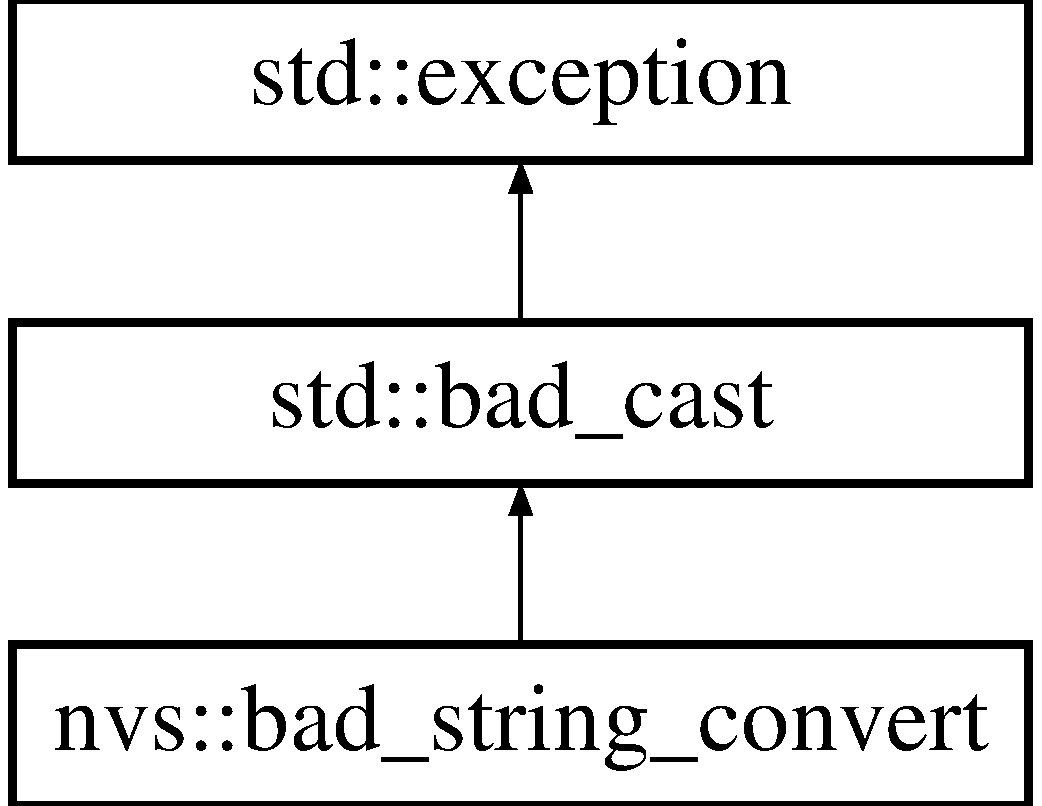
\includegraphics[height=3.000000cm]{classnvs_1_1bad__string__convert}
\end{center}
\end{figure}
\subsection*{Public Member Functions}
\begin{DoxyCompactItemize}
\item 
\hypertarget{classnvs_1_1bad__string__convert_a350e4edfec1e675896be8e1e303b4706}{virtual \hyperlink{classnvs_1_1bad__string__convert_a350e4edfec1e675896be8e1e303b4706}{$\sim$bad\+\_\+string\+\_\+convert} ()=default}\label{classnvs_1_1bad__string__convert_a350e4edfec1e675896be8e1e303b4706}

\begin{DoxyCompactList}\small\item\em Destructeur par défaut. \end{DoxyCompactList}\item 
virtual const char $\ast$ \hyperlink{classnvs_1_1bad__string__convert_a086b280c9feeae9b0548665da4abaee8}{what} () const   throw ()
\begin{DoxyCompactList}\small\item\em Retourne une description de l'erreur rencontrée. \end{DoxyCompactList}\end{DoxyCompactItemize}


\subsection{Detailed Description}
Classe d'exception utilisée lors des conversions depuis une {\ttfamily std\+::string}. 

Levée par \hyperlink{namespacenvs_a96cda281b4b965c337c5a6bda3262a51}{nvs\+::from\+String}. 

\subsection{Member Function Documentation}
\hypertarget{classnvs_1_1bad__string__convert_a086b280c9feeae9b0548665da4abaee8}{\index{nvs\+::bad\+\_\+string\+\_\+convert@{nvs\+::bad\+\_\+string\+\_\+convert}!what@{what}}
\index{what@{what}!nvs\+::bad\+\_\+string\+\_\+convert@{nvs\+::bad\+\_\+string\+\_\+convert}}
\subsubsection[{what}]{\setlength{\rightskip}{0pt plus 5cm}virtual const char$\ast$ nvs\+::bad\+\_\+string\+\_\+convert\+::what (
\begin{DoxyParamCaption}
{}
\end{DoxyParamCaption}
) const throw  ) \hspace{0.3cm}{\ttfamily [inline]}, {\ttfamily [virtual]}}}\label{classnvs_1_1bad__string__convert_a086b280c9feeae9b0548665da4abaee8}


Retourne une description de l'erreur rencontrée. 

En fait, retourne toujours la chaîne de caractères \+: {\ttfamily nvs\+::bad\+\_\+string\+\_\+convert}. Pas très utile donc...

\begin{DoxyReturn}{Returns}
La chaîne de caractères \+: {\ttfamily nvs\+::bad\+\_\+string\+\_\+convert}. 
\end{DoxyReturn}


The documentation for this class was generated from the following file\+:\begin{DoxyCompactItemize}
\item 
src/libs/\hyperlink{stringConvert_8hpp}{string\+Convert.\+hpp}\end{DoxyCompactItemize}

\hypertarget{classConnectN}{\section{Connect\+N Class Reference}
\label{classConnectN}\index{Connect\+N@{Connect\+N}}
}


The \hyperlink{classConnectN}{Connect\+N} game.  




{\ttfamily \#include $<$Connect\+N.\+h$>$}

\subsection*{Public Types}
\begin{DoxyCompactItemize}
\item 
enum \{ \hyperlink{classConnectN_afbc5b3f1ce192977e53400984d532d1ba8dabbd51219a23e08073e6c946755bc8}{D\+E\+F\+A\+U\+L\+T\+\_\+\+P\+O\+W\+E\+R} = 4, 
\hyperlink{classConnectN_afbc5b3f1ce192977e53400984d532d1bae24544d9408db101c664328a5c00137c}{D\+E\+F\+A\+U\+L\+T\+\_\+\+L\+I\+N\+E} = 6, 
\hyperlink{classConnectN_afbc5b3f1ce192977e53400984d532d1ba1ebbe9aa1e009f66a6c5c022f5ee0e50}{D\+E\+F\+A\+U\+L\+T\+\_\+\+C\+O\+L\+U\+M\+N} = 7
 \}
\end{DoxyCompactItemize}
\subsection*{Public Member Functions}
\begin{DoxyCompactItemize}
\item 
\hyperlink{classConnectN_ae4c655de7116f32bf84ba01d8fa09455}{Connect\+N} ()
\begin{DoxyCompactList}\small\item\em Default \hyperlink{classConnectN}{Connect\+N} constructor. \end{DoxyCompactList}\item 
\hyperlink{classConnectN_aef059ecefe9eafeae4c9fa8806b14a43}{Connect\+N} (unsigned \hyperlink{classConnectN_a297db626a235c0bebfc276cb4b818cd6}{power}, unsigned \hyperlink{classConnectN_afc8593800090e0d19532e9bdeefabac9}{line}, unsigned \hyperlink{classConnectN_a40cc2c86197b7502276490ec1399b0b4}{column})
\begin{DoxyCompactList}\small\item\em Custom \hyperlink{classConnectN}{Connect\+N} constructor. \end{DoxyCompactList}\item 
void \hyperlink{classConnectN_aeacffa2ecadbf102749c668073df72ad}{enroll} (const \hyperlink{classPlayer}{Player} $\ast$player)
\begin{DoxyCompactList}\small\item\em Enroll a player. \end{DoxyCompactList}\item 
void \hyperlink{classConnectN_a1bb5f50f1e29d34c48cc9231afe76af6}{play} (unsigned \hyperlink{classConnectN_a40cc2c86197b7502276490ec1399b0b4}{column})
\begin{DoxyCompactList}\small\item\em Play at the given column. \end{DoxyCompactList}\item 
unsigned \hyperlink{classConnectN_a297db626a235c0bebfc276cb4b818cd6}{power} () const 
\begin{DoxyCompactList}\small\item\em Return the number of pieces to align. \end{DoxyCompactList}\item 
unsigned \hyperlink{classConnectN_afc8593800090e0d19532e9bdeefabac9}{line} () const 
\begin{DoxyCompactList}\small\item\em Return the number of lines. \end{DoxyCompactList}\item 
unsigned \hyperlink{classConnectN_a40cc2c86197b7502276490ec1399b0b4}{column} () const 
\begin{DoxyCompactList}\small\item\em Return the number of columns. \end{DoxyCompactList}\item 
bool \hyperlink{classConnectN_a52e76a27a6ae77edcf65a24c67cfe83a}{started} () const 
\begin{DoxyCompactList}\small\item\em Check if the game is started. \end{DoxyCompactList}\item 
bool \hyperlink{classConnectN_aea9a731ecfed4ec40af668de60b8b311}{finished} () const 
\begin{DoxyCompactList}\small\item\em Check if the game is finished. \end{DoxyCompactList}\item 
const \hyperlink{classPlayer}{Player} $\ast$ \hyperlink{classConnectN_a234490fe29ede9056f1fadc4dddd087b}{winner} () const 
\begin{DoxyCompactList}\small\item\em Return the winner. \end{DoxyCompactList}\item 
const \hyperlink{classPlayer}{Player} $\ast$ \hyperlink{classConnectN_abaedcab14c58c5fc5621f76a271a7744}{active\+Player} () const 
\begin{DoxyCompactList}\small\item\em Return the active player. \end{DoxyCompactList}\item 
const std\+::array$<$ std\+::pair\\*
$<$ const \hyperlink{classPlayer}{Player} $\ast$, \hyperlink{Color_8h_ab87bacfdad76e61b9412d7124be44c1c}{Color} $>$, 2 $>$ \hyperlink{classConnectN_af9520dc89721a2702c8f6747d3711c44}{players} () const 
\begin{DoxyCompactList}\small\item\em Return an array of players, associated with their color. \end{DoxyCompactList}\item 
\hyperlink{Color_8h_ab87bacfdad76e61b9412d7124be44c1c}{Color} \hyperlink{classConnectN_a1f044297c006496edb2fe9f2cdc61f2d}{color} (const \hyperlink{classPlayer}{Player} $\ast$) const 
\begin{DoxyCompactList}\small\item\em Return the color of the given player. \end{DoxyCompactList}\item 
const std\+::vector$<$ std\+::vector\\*
$<$ \hyperlink{Color_8h_ab87bacfdad76e61b9412d7124be44c1c}{Color} $>$ $>$ \& \hyperlink{classConnectN_adc7bac377c8a1ff4976a424bdf6627c8}{board} () const 
\begin{DoxyCompactList}\small\item\em Return the game board. \end{DoxyCompactList}\end{DoxyCompactItemize}
\subsection*{Static Public Attributes}
\begin{DoxyCompactItemize}
\item 
\hypertarget{classConnectN_a0098050ba1e1691aa2bab3eeacd127be}{static const unsigned \hyperlink{classConnectN_a0098050ba1e1691aa2bab3eeacd127be}{M\+I\+N\+\_\+\+P\+O\+W\+E\+R} = 3}\label{classConnectN_a0098050ba1e1691aa2bab3eeacd127be}

\begin{DoxyCompactList}\small\item\em Minimum allowed power. \end{DoxyCompactList}\item 
\hypertarget{classConnectN_a785bea2a4b4bf7b12d5611afc309096b}{static const unsigned \hyperlink{classConnectN_a785bea2a4b4bf7b12d5611afc309096b}{M\+A\+X\+\_\+\+P\+O\+W\+E\+R} = 10}\label{classConnectN_a785bea2a4b4bf7b12d5611afc309096b}

\begin{DoxyCompactList}\small\item\em Maximum allowed power. \end{DoxyCompactList}\item 
\hypertarget{classConnectN_aba6b11a59052663b23cb2a9611d25d2f}{static const unsigned \hyperlink{classConnectN_aba6b11a59052663b23cb2a9611d25d2f}{D\+E\+L\+T\+A\+\_\+\+L\+I\+N\+E} = \hyperlink{classConnectN_a785bea2a4b4bf7b12d5611afc309096b}{M\+A\+X\+\_\+\+P\+O\+W\+E\+R} + 10}\label{classConnectN_aba6b11a59052663b23cb2a9611d25d2f}

\begin{DoxyCompactList}\small\item\em Maximum line number depending on the maximum allowed power. \end{DoxyCompactList}\item 
\hypertarget{classConnectN_a111b3987f792f8dca47d857f3f88ba61}{static const unsigned \hyperlink{classConnectN_a111b3987f792f8dca47d857f3f88ba61}{D\+E\+L\+T\+A\+\_\+\+C\+O\+L\+U\+M\+N} = \hyperlink{classConnectN_a785bea2a4b4bf7b12d5611afc309096b}{M\+A\+X\+\_\+\+P\+O\+W\+E\+R} + 10}\label{classConnectN_a111b3987f792f8dca47d857f3f88ba61}

\begin{DoxyCompactList}\small\item\em Maximum column number depending on the maximum allowed power. \end{DoxyCompactList}\end{DoxyCompactItemize}


\subsection{Detailed Description}
The \hyperlink{classConnectN}{Connect\+N} game. 

\subsection{Member Enumeration Documentation}
\hypertarget{classConnectN_afbc5b3f1ce192977e53400984d532d1b}{\subsubsection[{anonymous enum}]{\setlength{\rightskip}{0pt plus 5cm}anonymous enum}}\label{classConnectN_afbc5b3f1ce192977e53400984d532d1b}
\begin{Desc}
\item[Enumerator]\par
\begin{description}
\index{D\+E\+F\+A\+U\+L\+T\+\_\+\+P\+O\+W\+E\+R@{D\+E\+F\+A\+U\+L\+T\+\_\+\+P\+O\+W\+E\+R}!Connect\+N@{Connect\+N}}\index{Connect\+N@{Connect\+N}!D\+E\+F\+A\+U\+L\+T\+\_\+\+P\+O\+W\+E\+R@{D\+E\+F\+A\+U\+L\+T\+\_\+\+P\+O\+W\+E\+R}}\item[{\em 
\hypertarget{classConnectN_afbc5b3f1ce192977e53400984d532d1ba8dabbd51219a23e08073e6c946755bc8}{D\+E\+F\+A\+U\+L\+T\+\_\+\+P\+O\+W\+E\+R}\label{classConnectN_afbc5b3f1ce192977e53400984d532d1ba8dabbd51219a23e08073e6c946755bc8}
}]Default power. \index{D\+E\+F\+A\+U\+L\+T\+\_\+\+L\+I\+N\+E@{D\+E\+F\+A\+U\+L\+T\+\_\+\+L\+I\+N\+E}!Connect\+N@{Connect\+N}}\index{Connect\+N@{Connect\+N}!D\+E\+F\+A\+U\+L\+T\+\_\+\+L\+I\+N\+E@{D\+E\+F\+A\+U\+L\+T\+\_\+\+L\+I\+N\+E}}\item[{\em 
\hypertarget{classConnectN_afbc5b3f1ce192977e53400984d532d1bae24544d9408db101c664328a5c00137c}{D\+E\+F\+A\+U\+L\+T\+\_\+\+L\+I\+N\+E}\label{classConnectN_afbc5b3f1ce192977e53400984d532d1bae24544d9408db101c664328a5c00137c}
}]Default line. \index{D\+E\+F\+A\+U\+L\+T\+\_\+\+C\+O\+L\+U\+M\+N@{D\+E\+F\+A\+U\+L\+T\+\_\+\+C\+O\+L\+U\+M\+N}!Connect\+N@{Connect\+N}}\index{Connect\+N@{Connect\+N}!D\+E\+F\+A\+U\+L\+T\+\_\+\+C\+O\+L\+U\+M\+N@{D\+E\+F\+A\+U\+L\+T\+\_\+\+C\+O\+L\+U\+M\+N}}\item[{\em 
\hypertarget{classConnectN_afbc5b3f1ce192977e53400984d532d1ba1ebbe9aa1e009f66a6c5c022f5ee0e50}{D\+E\+F\+A\+U\+L\+T\+\_\+\+C\+O\+L\+U\+M\+N}\label{classConnectN_afbc5b3f1ce192977e53400984d532d1ba1ebbe9aa1e009f66a6c5c022f5ee0e50}
}]Default column. \end{description}
\end{Desc}


\subsection{Constructor \& Destructor Documentation}
\hypertarget{classConnectN_ae4c655de7116f32bf84ba01d8fa09455}{\index{Connect\+N@{Connect\+N}!Connect\+N@{Connect\+N}}
\index{Connect\+N@{Connect\+N}!Connect\+N@{Connect\+N}}
\subsubsection[{Connect\+N}]{\setlength{\rightskip}{0pt plus 5cm}Connect\+N\+::\+Connect\+N (
\begin{DoxyParamCaption}
{}
\end{DoxyParamCaption}
)}}\label{classConnectN_ae4c655de7116f32bf84ba01d8fa09455}


Default \hyperlink{classConnectN}{Connect\+N} constructor. 

D\+E\+F\+A\+U\+L\+T\+\_\+\+P\+O\+W\+E\+R, D\+E\+F\+A\+U\+L\+T\+\_\+\+L\+I\+N\+E and D\+E\+F\+A\+U\+L\+T\+\_\+\+C\+O\+L\+U\+M\+N are used as default values. \hypertarget{classConnectN_aef059ecefe9eafeae4c9fa8806b14a43}{\index{Connect\+N@{Connect\+N}!Connect\+N@{Connect\+N}}
\index{Connect\+N@{Connect\+N}!Connect\+N@{Connect\+N}}
\subsubsection[{Connect\+N}]{\setlength{\rightskip}{0pt plus 5cm}Connect\+N\+::\+Connect\+N (
\begin{DoxyParamCaption}
\item[{unsigned}]{power, }
\item[{unsigned}]{line, }
\item[{unsigned}]{column}
\end{DoxyParamCaption}
)}}\label{classConnectN_aef059ecefe9eafeae4c9fa8806b14a43}


Custom \hyperlink{classConnectN}{Connect\+N} constructor. 


\begin{DoxyParams}{Parameters}
{\em power} & number of pieces to align \\
\hline
{\em line} & number of lines of the board \\
\hline
{\em column} & number of columns of the board \\
\hline
\end{DoxyParams}


\subsection{Member Function Documentation}
\hypertarget{classConnectN_abaedcab14c58c5fc5621f76a271a7744}{\index{Connect\+N@{Connect\+N}!active\+Player@{active\+Player}}
\index{active\+Player@{active\+Player}!Connect\+N@{Connect\+N}}
\subsubsection[{active\+Player}]{\setlength{\rightskip}{0pt plus 5cm}const {\bf Player}$\ast$ Connect\+N\+::active\+Player (
\begin{DoxyParamCaption}
{}
\end{DoxyParamCaption}
) const}}\label{classConnectN_abaedcab14c58c5fc5621f76a271a7744}


Return the active player. 

\begin{DoxyReturn}{Returns}
the active player if any, {\ttfamily nullptr} otherwise 
\end{DoxyReturn}
\hypertarget{classConnectN_adc7bac377c8a1ff4976a424bdf6627c8}{\index{Connect\+N@{Connect\+N}!board@{board}}
\index{board@{board}!Connect\+N@{Connect\+N}}
\subsubsection[{board}]{\setlength{\rightskip}{0pt plus 5cm}const std\+::vector$<$std\+::vector$<${\bf Color}$>$ $>$\& Connect\+N\+::board (
\begin{DoxyParamCaption}
{}
\end{DoxyParamCaption}
) const}}\label{classConnectN_adc7bac377c8a1ff4976a424bdf6627c8}


Return the game board. 

\begin{DoxyReturn}{Returns}
the game board 
\end{DoxyReturn}
\hypertarget{classConnectN_a1f044297c006496edb2fe9f2cdc61f2d}{\index{Connect\+N@{Connect\+N}!color@{color}}
\index{color@{color}!Connect\+N@{Connect\+N}}
\subsubsection[{color}]{\setlength{\rightskip}{0pt plus 5cm}{\bf Color} Connect\+N\+::color (
\begin{DoxyParamCaption}
\item[{const {\bf Player} $\ast$}]{}
\end{DoxyParamCaption}
) const}}\label{classConnectN_a1f044297c006496edb2fe9f2cdc61f2d}


Return the color of the given player. 

\begin{DoxyReturn}{Returns}
the color of the given player 
\end{DoxyReturn}
\hypertarget{classConnectN_a40cc2c86197b7502276490ec1399b0b4}{\index{Connect\+N@{Connect\+N}!column@{column}}
\index{column@{column}!Connect\+N@{Connect\+N}}
\subsubsection[{column}]{\setlength{\rightskip}{0pt plus 5cm}unsigned Connect\+N\+::column (
\begin{DoxyParamCaption}
{}
\end{DoxyParamCaption}
) const}}\label{classConnectN_a40cc2c86197b7502276490ec1399b0b4}


Return the number of columns. 

\begin{DoxyReturn}{Returns}
the number of columns 
\end{DoxyReturn}
\hypertarget{classConnectN_aeacffa2ecadbf102749c668073df72ad}{\index{Connect\+N@{Connect\+N}!enroll@{enroll}}
\index{enroll@{enroll}!Connect\+N@{Connect\+N}}
\subsubsection[{enroll}]{\setlength{\rightskip}{0pt plus 5cm}void Connect\+N\+::enroll (
\begin{DoxyParamCaption}
\item[{const {\bf Player} $\ast$}]{player}
\end{DoxyParamCaption}
)}}\label{classConnectN_aeacffa2ecadbf102749c668073df72ad}


Enroll a player. 


\begin{DoxyParams}{Parameters}
{\em player} & the player to enroll \\
\hline
\end{DoxyParams}

\begin{DoxyExceptions}{Exceptions}
{\em std\+::invalid\+\_\+argument} & if the given player is already enrolled \\
\hline
{\em std\+::logic\+\_\+error} & if two players are already enrolled \\
\hline
\end{DoxyExceptions}
\hypertarget{classConnectN_aea9a731ecfed4ec40af668de60b8b311}{\index{Connect\+N@{Connect\+N}!finished@{finished}}
\index{finished@{finished}!Connect\+N@{Connect\+N}}
\subsubsection[{finished}]{\setlength{\rightskip}{0pt plus 5cm}bool Connect\+N\+::finished (
\begin{DoxyParamCaption}
{}
\end{DoxyParamCaption}
) const}}\label{classConnectN_aea9a731ecfed4ec40af668de60b8b311}


Check if the game is finished. 

\begin{DoxyReturn}{Returns}
{\ttfamily true} if the game is finished, {\ttfamily false} otherwise 
\end{DoxyReturn}
\hypertarget{classConnectN_afc8593800090e0d19532e9bdeefabac9}{\index{Connect\+N@{Connect\+N}!line@{line}}
\index{line@{line}!Connect\+N@{Connect\+N}}
\subsubsection[{line}]{\setlength{\rightskip}{0pt plus 5cm}unsigned Connect\+N\+::line (
\begin{DoxyParamCaption}
{}
\end{DoxyParamCaption}
) const}}\label{classConnectN_afc8593800090e0d19532e9bdeefabac9}


Return the number of lines. 

\begin{DoxyReturn}{Returns}
the number of lines 
\end{DoxyReturn}
\hypertarget{classConnectN_a1bb5f50f1e29d34c48cc9231afe76af6}{\index{Connect\+N@{Connect\+N}!play@{play}}
\index{play@{play}!Connect\+N@{Connect\+N}}
\subsubsection[{play}]{\setlength{\rightskip}{0pt plus 5cm}void Connect\+N\+::play (
\begin{DoxyParamCaption}
\item[{unsigned}]{column}
\end{DoxyParamCaption}
)}}\label{classConnectN_a1bb5f50f1e29d34c48cc9231afe76af6}


Play at the given column. 

This method tries to drop a piece in the column given as parameter. If it works, the board is checked to see if N pieces are aligned. If true, the winner is the current player; if not, the other player becomes the current player, and the game continues. 
\begin{DoxyParams}{Parameters}
{\em column} & the column where to play \\
\hline
\end{DoxyParams}

\begin{DoxyExceptions}{Exceptions}
{\em std\+::logic\+\_\+error} & if
\begin{DoxyItemize}
\item the game is not started
\item the game is finished 
\end{DoxyItemize}\\
\hline
{\em std\+::out\+\_\+of\+\_\+range} & if
\begin{DoxyItemize}
\item the column is full
\item the column given as parameter is out of the board 
\end{DoxyItemize}\\
\hline
\end{DoxyExceptions}
\hypertarget{classConnectN_af9520dc89721a2702c8f6747d3711c44}{\index{Connect\+N@{Connect\+N}!players@{players}}
\index{players@{players}!Connect\+N@{Connect\+N}}
\subsubsection[{players}]{\setlength{\rightskip}{0pt plus 5cm}const std\+::array$<$std\+::pair$<$const {\bf Player} $\ast$, {\bf Color}$>$, 2$>$ Connect\+N\+::players (
\begin{DoxyParamCaption}
{}
\end{DoxyParamCaption}
) const}}\label{classConnectN_af9520dc89721a2702c8f6747d3711c44}


Return an array of players, associated with their color. 

\begin{DoxyReturn}{Returns}
an array of players, associated with their color 
\end{DoxyReturn}
\hypertarget{classConnectN_a297db626a235c0bebfc276cb4b818cd6}{\index{Connect\+N@{Connect\+N}!power@{power}}
\index{power@{power}!Connect\+N@{Connect\+N}}
\subsubsection[{power}]{\setlength{\rightskip}{0pt plus 5cm}unsigned Connect\+N\+::power (
\begin{DoxyParamCaption}
{}
\end{DoxyParamCaption}
) const}}\label{classConnectN_a297db626a235c0bebfc276cb4b818cd6}


Return the number of pieces to align. 

\begin{DoxyReturn}{Returns}
the number of pieces to align 
\end{DoxyReturn}
\hypertarget{classConnectN_a52e76a27a6ae77edcf65a24c67cfe83a}{\index{Connect\+N@{Connect\+N}!started@{started}}
\index{started@{started}!Connect\+N@{Connect\+N}}
\subsubsection[{started}]{\setlength{\rightskip}{0pt plus 5cm}bool Connect\+N\+::started (
\begin{DoxyParamCaption}
{}
\end{DoxyParamCaption}
) const}}\label{classConnectN_a52e76a27a6ae77edcf65a24c67cfe83a}


Check if the game is started. 

\begin{DoxyReturn}{Returns}
{\ttfamily true} if the game is started, {\ttfamily false} otherwise 
\end{DoxyReturn}
\hypertarget{classConnectN_a234490fe29ede9056f1fadc4dddd087b}{\index{Connect\+N@{Connect\+N}!winner@{winner}}
\index{winner@{winner}!Connect\+N@{Connect\+N}}
\subsubsection[{winner}]{\setlength{\rightskip}{0pt plus 5cm}const {\bf Player}$\ast$ Connect\+N\+::winner (
\begin{DoxyParamCaption}
{}
\end{DoxyParamCaption}
) const}}\label{classConnectN_a234490fe29ede9056f1fadc4dddd087b}


Return the winner. 

\begin{DoxyReturn}{Returns}
the winner if any, {\ttfamily nullptr} otherwise 
\end{DoxyReturn}


The documentation for this class was generated from the following files\+:\begin{DoxyCompactItemize}
\item 
src/\hyperlink{ConnectN_8h}{Connect\+N.\+h}\item 
src/Connect\+N.\+cpp\end{DoxyCompactItemize}

\hypertarget{classPlayer}{\section{Player Class Reference}
\label{classPlayer}\index{Player@{Player}}
}


A \hyperlink{classConnectN}{Connect\+N} player.  




{\ttfamily \#include $<$Player.\+h$>$}

\subsection*{Public Member Functions}
\begin{DoxyCompactItemize}
\item 
\hyperlink{classPlayer_a45fa04a2a4ff9235e6c100b7c6ab232a}{Player} (const std\+::string \&\hyperlink{classPlayer_a2e37623a770cfad59be24589dee744de}{name})
\begin{DoxyCompactList}\small\item\em \hyperlink{classPlayer}{Player} constructor. \end{DoxyCompactList}\item 
const std\+::string \& \hyperlink{classPlayer_a2e37623a770cfad59be24589dee744de}{name} () const 
\begin{DoxyCompactList}\small\item\em Return the name of the player. \end{DoxyCompactList}\end{DoxyCompactItemize}


\subsection{Detailed Description}
A \hyperlink{classConnectN}{Connect\+N} player. 

\subsection{Constructor \& Destructor Documentation}
\hypertarget{classPlayer_a45fa04a2a4ff9235e6c100b7c6ab232a}{\index{Player@{Player}!Player@{Player}}
\index{Player@{Player}!Player@{Player}}
\subsubsection[{Player}]{\setlength{\rightskip}{0pt plus 5cm}Player\+::\+Player (
\begin{DoxyParamCaption}
\item[{const std\+::string \&}]{name}
\end{DoxyParamCaption}
)}}\label{classPlayer_a45fa04a2a4ff9235e6c100b7c6ab232a}


\hyperlink{classPlayer}{Player} constructor. 


\begin{DoxyParams}{Parameters}
{\em name} & the name of the player \\
\hline
\end{DoxyParams}


\subsection{Member Function Documentation}
\hypertarget{classPlayer_a2e37623a770cfad59be24589dee744de}{\index{Player@{Player}!name@{name}}
\index{name@{name}!Player@{Player}}
\subsubsection[{name}]{\setlength{\rightskip}{0pt plus 5cm}const std\+::string \& Player\+::name (
\begin{DoxyParamCaption}
{}
\end{DoxyParamCaption}
) const}}\label{classPlayer_a2e37623a770cfad59be24589dee744de}


Return the name of the player. 

\begin{DoxyReturn}{Returns}
the name of the player 
\end{DoxyReturn}


The documentation for this class was generated from the following files\+:\begin{DoxyCompactItemize}
\item 
src/\hyperlink{Player_8h}{Player.\+h}\item 
src/Player.\+cpp\end{DoxyCompactItemize}

\chapter{File Documentation}
\hypertarget{Color_8h}{\section{src/\+Color.h File Reference}
\label{Color_8h}\index{src/\+Color.\+h@{src/\+Color.\+h}}
}


Color enum class definition.  


{\ttfamily \#include $<$ostream$>$}\\*
{\ttfamily \#include $<$string$>$}\\*
\subsection*{Enumerations}
\begin{DoxyCompactItemize}
\item 
enum \hyperlink{Color_8h_ab87bacfdad76e61b9412d7124be44c1c}{Color} \{ \hyperlink{Color_8h_ab87bacfdad76e61b9412d7124be44c1cab50339a10e1de285ac99d4c3990b8693}{Color\+::\+N\+O\+N\+E}, 
\hyperlink{Color_8h_ab87bacfdad76e61b9412d7124be44c1ca08d0012388564e95c3b4a7407cf04965}{Color\+::\+B\+L\+A\+C\+K}, 
\hyperlink{Color_8h_ab87bacfdad76e61b9412d7124be44c1cab5bf627e448384cf3a4c35121ca6008d}{Color\+::\+W\+H\+I\+T\+E}
 \}
\begin{DoxyCompactList}\small\item\em The Color enum class. \end{DoxyCompactList}\end{DoxyCompactItemize}
\subsection*{Functions}
\begin{DoxyCompactItemize}
\item 
std\+::string \hyperlink{Color_8h_a6c449369b82877cb7a7b3c9a2665d086}{to\+\_\+string} (\hyperlink{Color_8h_ab87bacfdad76e61b9412d7124be44c1c}{Color} color)
\begin{DoxyCompactList}\small\item\em to\+\_\+string \end{DoxyCompactList}\item 
std\+::ostream \& \hyperlink{Color_8h_a410ecbc348077df3a205c1f90d787fd3}{operator$<$$<$} (std\+::ostream \&out, \hyperlink{Color_8h_ab87bacfdad76e61b9412d7124be44c1c}{Color} in)
\begin{DoxyCompactList}\small\item\em Color output stream operator. \end{DoxyCompactList}\end{DoxyCompactItemize}


\subsection{Detailed Description}
Color enum class definition. 



\subsection{Enumeration Type Documentation}
\hypertarget{Color_8h_ab87bacfdad76e61b9412d7124be44c1c}{\index{Color.\+h@{Color.\+h}!Color@{Color}}
\index{Color@{Color}!Color.\+h@{Color.\+h}}
\subsubsection[{Color}]{\setlength{\rightskip}{0pt plus 5cm}enum {\bf Color}\hspace{0.3cm}{\ttfamily [strong]}}}\label{Color_8h_ab87bacfdad76e61b9412d7124be44c1c}


The Color enum class. 

\begin{Desc}
\item[Enumerator]\par
\begin{description}
\index{N\+O\+N\+E@{N\+O\+N\+E}!Color.\+h@{Color.\+h}}\index{Color.\+h@{Color.\+h}!N\+O\+N\+E@{N\+O\+N\+E}}\item[{\em 
\hypertarget{Color_8h_ab87bacfdad76e61b9412d7124be44c1cab50339a10e1de285ac99d4c3990b8693}{N\+O\+N\+E}\label{Color_8h_ab87bacfdad76e61b9412d7124be44c1cab50339a10e1de285ac99d4c3990b8693}
}]an empty color \index{B\+L\+A\+C\+K@{B\+L\+A\+C\+K}!Color.\+h@{Color.\+h}}\index{Color.\+h@{Color.\+h}!B\+L\+A\+C\+K@{B\+L\+A\+C\+K}}\item[{\em 
\hypertarget{Color_8h_ab87bacfdad76e61b9412d7124be44c1ca08d0012388564e95c3b4a7407cf04965}{B\+L\+A\+C\+K}\label{Color_8h_ab87bacfdad76e61b9412d7124be44c1ca08d0012388564e95c3b4a7407cf04965}
}]a black piece \index{W\+H\+I\+T\+E@{W\+H\+I\+T\+E}!Color.\+h@{Color.\+h}}\index{Color.\+h@{Color.\+h}!W\+H\+I\+T\+E@{W\+H\+I\+T\+E}}\item[{\em 
\hypertarget{Color_8h_ab87bacfdad76e61b9412d7124be44c1cab5bf627e448384cf3a4c35121ca6008d}{W\+H\+I\+T\+E}\label{Color_8h_ab87bacfdad76e61b9412d7124be44c1cab5bf627e448384cf3a4c35121ca6008d}
}]a white piece \end{description}
\end{Desc}


\subsection{Function Documentation}
\hypertarget{Color_8h_a410ecbc348077df3a205c1f90d787fd3}{\index{Color.\+h@{Color.\+h}!operator$<$$<$@{operator$<$$<$}}
\index{operator$<$$<$@{operator$<$$<$}!Color.\+h@{Color.\+h}}
\subsubsection[{operator$<$$<$}]{\setlength{\rightskip}{0pt plus 5cm}std\+::ostream\& operator$<$$<$ (
\begin{DoxyParamCaption}
\item[{std\+::ostream \&}]{out, }
\item[{{\bf Color}}]{in}
\end{DoxyParamCaption}
)}}\label{Color_8h_a410ecbc348077df3a205c1f90d787fd3}


Color output stream operator. 


\begin{DoxyParams}{Parameters}
{\em out} & the output stream \\
\hline
{\em in} & the color \\
\hline
\end{DoxyParams}
\begin{DoxyReturn}{Returns}
the string representation of the color 
\end{DoxyReturn}
\hypertarget{Color_8h_a6c449369b82877cb7a7b3c9a2665d086}{\index{Color.\+h@{Color.\+h}!to\+\_\+string@{to\+\_\+string}}
\index{to\+\_\+string@{to\+\_\+string}!Color.\+h@{Color.\+h}}
\subsubsection[{to\+\_\+string}]{\setlength{\rightskip}{0pt plus 5cm}std\+::string to\+\_\+string (
\begin{DoxyParamCaption}
\item[{{\bf Color}}]{color}
\end{DoxyParamCaption}
)}}\label{Color_8h_a6c449369b82877cb7a7b3c9a2665d086}


to\+\_\+string 


\begin{DoxyParams}{Parameters}
{\em color} & the color \\
\hline
\end{DoxyParams}
\begin{DoxyReturn}{Returns}
the string representation of the color 
\end{DoxyReturn}

\hypertarget{ConnectN_8h}{\section{src/\+Connect\+N.h File Reference}
\label{ConnectN_8h}\index{src/\+Connect\+N.\+h@{src/\+Connect\+N.\+h}}
}


\hyperlink{classConnectN}{Connect\+N} class definition.  


{\ttfamily \#include $<$vector$>$}\\*
{\ttfamily \#include $<$array$>$}\\*
{\ttfamily \#include $<$string$>$}\\*
{\ttfamily \#include $<$sstream$>$}\\*
{\ttfamily \#include \char`\"{}Player.\+h\char`\"{}}\\*
{\ttfamily \#include \char`\"{}Color.\+h\char`\"{}}\\*
\subsection*{Classes}
\begin{DoxyCompactItemize}
\item 
class \hyperlink{classConnectN}{Connect\+N}
\begin{DoxyCompactList}\small\item\em The \hyperlink{classConnectN}{Connect\+N} game. \end{DoxyCompactList}\end{DoxyCompactItemize}
\subsection*{Functions}
\begin{DoxyCompactItemize}
\item 
std\+::string \hyperlink{ConnectN_8h_ab289e8ccf1eb4cb4ebccdc057c43e5e7}{to\+\_\+string} (const \hyperlink{classConnectN}{Connect\+N} \&game)
\begin{DoxyCompactList}\small\item\em to\+\_\+string \end{DoxyCompactList}\item 
std\+::ostream \& \hyperlink{ConnectN_8h_a4c1055002b6b515b1ea3ea3d98eca620}{operator$<$$<$} (std\+::ostream \&out, \hyperlink{classConnectN}{Connect\+N} in)
\begin{DoxyCompactList}\small\item\em \hyperlink{classConnectN}{Connect\+N} output stream operator. \end{DoxyCompactList}\end{DoxyCompactItemize}


\subsection{Detailed Description}
\hyperlink{classConnectN}{Connect\+N} class definition. 



\subsection{Function Documentation}
\hypertarget{ConnectN_8h_a4c1055002b6b515b1ea3ea3d98eca620}{\index{Connect\+N.\+h@{Connect\+N.\+h}!operator$<$$<$@{operator$<$$<$}}
\index{operator$<$$<$@{operator$<$$<$}!Connect\+N.\+h@{Connect\+N.\+h}}
\subsubsection[{operator$<$$<$}]{\setlength{\rightskip}{0pt plus 5cm}std\+::ostream\& operator$<$$<$ (
\begin{DoxyParamCaption}
\item[{std\+::ostream \&}]{out, }
\item[{{\bf Connect\+N}}]{in}
\end{DoxyParamCaption}
)}}\label{ConnectN_8h_a4c1055002b6b515b1ea3ea3d98eca620}


\hyperlink{classConnectN}{Connect\+N} output stream operator. 


\begin{DoxyParams}{Parameters}
{\em out} & the output stream \\
\hline
{\em in} & the \hyperlink{classConnectN}{Connect\+N} game \\
\hline
\end{DoxyParams}
\begin{DoxyReturn}{Returns}
the string representation of the \hyperlink{classConnectN}{Connect\+N} game 
\end{DoxyReturn}
\hypertarget{ConnectN_8h_ab289e8ccf1eb4cb4ebccdc057c43e5e7}{\index{Connect\+N.\+h@{Connect\+N.\+h}!to\+\_\+string@{to\+\_\+string}}
\index{to\+\_\+string@{to\+\_\+string}!Connect\+N.\+h@{Connect\+N.\+h}}
\subsubsection[{to\+\_\+string}]{\setlength{\rightskip}{0pt plus 5cm}std\+::string to\+\_\+string (
\begin{DoxyParamCaption}
\item[{const {\bf Connect\+N} \&}]{game}
\end{DoxyParamCaption}
)}}\label{ConnectN_8h_ab289e8ccf1eb4cb4ebccdc057c43e5e7}


to\+\_\+string 


\begin{DoxyParams}{Parameters}
{\em game} & the game \\
\hline
\end{DoxyParams}
\begin{DoxyReturn}{Returns}
the string representation of the \hyperlink{classConnectN}{Connect\+N} game 
\end{DoxyReturn}

\hypertarget{keyboard_8hpp}{\section{src/libs/keyboard.hpp File Reference}
\label{keyboard_8hpp}\index{src/libs/keyboard.\+hpp@{src/libs/keyboard.\+hpp}}
}


Contient les modèles de fonctions pour lire des données au clavier.  


{\ttfamily \#include \char`\"{}string\+Convert.\+hpp\char`\"{}}\\*
{\ttfamily \#include $<$string$>$}\\*
{\ttfamily \#include $<$iostream$>$}\\*
\subsection*{Namespaces}
\begin{DoxyCompactItemize}
\item 
 \hyperlink{namespacenvs}{nvs}
\begin{DoxyCompactList}\small\item\em Espace de nom de Nicolas Vansteenkiste. \end{DoxyCompactList}\end{DoxyCompactItemize}
\subsection*{Functions}
\begin{DoxyCompactItemize}
\item 
{\footnotesize template$<$typename T $>$ }\\T \hyperlink{namespacenvs_a67222c9b17e02e6d95a7559f92ec4daf}{nvs\+::line\+From\+Kbd} (T \&t, bool iw=false)
\begin{DoxyCompactList}\small\item\em Lit toute une ligne au clavier et en extrait une seule donnée. \end{DoxyCompactList}\item 
{\footnotesize template$<$typename T $>$ }\\T \hyperlink{namespacenvs_a5c923479773c4d277d92d9e7a75b4567}{nvs\+::line\+From\+Kbd} (bool iw=false)
\begin{DoxyCompactList}\small\item\em Lit toute une ligne au clavier et en extrait une seule donnée. \end{DoxyCompactList}\end{DoxyCompactItemize}


\subsection{Detailed Description}
Contient les modèles de fonctions pour lire des données au clavier. 

\begin{DoxyAuthor}{Author}
nvs 
\end{DoxyAuthor}

\hypertarget{randomgenerator_8hpp}{\section{src/libs/randomgenerator.hpp File Reference}
\label{randomgenerator_8hpp}\index{src/libs/randomgenerator.\+hpp@{src/libs/randomgenerator.\+hpp}}
}


Définitions de fonctions conviviales pour générer des séquences pseudo-\/aléatoires.  


{\ttfamily \#include $<$random$>$}\\*
{\ttfamily \#include $<$limits$>$}\\*
{\ttfamily \#include $<$stdexcept$>$}\\*
{\ttfamily \#include $<$ctime$>$}\\*
\subsection*{Namespaces}
\begin{DoxyCompactItemize}
\item 
 \hyperlink{namespacenvs}{nvs}
\begin{DoxyCompactList}\small\item\em Espace de nom de Nicolas Vansteenkiste. \end{DoxyCompactList}\end{DoxyCompactItemize}
\subsection*{Functions}
\begin{DoxyCompactItemize}
\item 
{\footnotesize template$<$typename T $>$ }\\T \hyperlink{namespacenvs_aeb20a15a022be7b92a30006fcd03ffca}{nvs\+::random\+\_\+integer} (T min=std\+::numeric\+\_\+limits$<$ T $>$\+::min(), T max=std\+::numeric\+\_\+limits$<$ T $>$\+::max())
\begin{DoxyCompactList}\small\item\em Générateur d'entiers aléatoires. \end{DoxyCompactList}\end{DoxyCompactItemize}


\subsection{Detailed Description}
Définitions de fonctions conviviales pour générer des séquences pseudo-\/aléatoires. 


\hypertarget{stringConvert_8hpp}{\section{src/libs/string\+Convert.hpp File Reference}
\label{stringConvert_8hpp}\index{src/libs/string\+Convert.\+hpp@{src/libs/string\+Convert.\+hpp}}
}


Contient les modèles de fonctions pour convertir depuis et vers une {\ttfamily string} standard.  


{\ttfamily \#include $<$string$>$}\\*
{\ttfamily \#include $<$sstream$>$}\\*
{\ttfamily \#include $<$typeinfo$>$}\\*
\subsection*{Classes}
\begin{DoxyCompactItemize}
\item 
class \hyperlink{classnvs_1_1bad__string__convert}{nvs\+::bad\+\_\+string\+\_\+convert}
\begin{DoxyCompactList}\small\item\em Classe d'exception utilisée lors des conversions depuis une {\ttfamily std\+::string}. \end{DoxyCompactList}\end{DoxyCompactItemize}
\subsection*{Namespaces}
\begin{DoxyCompactItemize}
\item 
 \hyperlink{namespacenvs}{nvs}
\begin{DoxyCompactList}\small\item\em Espace de nom de Nicolas Vansteenkiste. \end{DoxyCompactList}\end{DoxyCompactItemize}
\subsection*{Functions}
\begin{DoxyCompactItemize}
\item 
{\footnotesize template$<$typename T $>$ }\\std\+::string \hyperlink{namespacenvs_aee50f16a11273a42501cb44b7a31610d}{nvs\+::to\+String} (const T \&in)
\begin{DoxyCompactList}\small\item\em Modèle de fonction de conversion d'un type quelconque vers une {\ttfamily string}. \end{DoxyCompactList}\item 
{\footnotesize template$<$typename T $>$ }\\T \hyperlink{namespacenvs_a96cda281b4b965c337c5a6bda3262a51}{nvs\+::from\+String} (T \&t, const std\+::string \&s, bool iw=false)
\begin{DoxyCompactList}\small\item\em Modèle de fonction de conversion d'une {\ttfamily string} vers un type quelconque {\itshape sauf} {\ttfamily char} et {\ttfamily char $\ast$}. \end{DoxyCompactList}\item 
{\footnotesize template$<$typename T $>$ }\\T \hyperlink{namespacenvs_a468a98727d8c71fb9e39bd6cf450b11c}{nvs\+::from\+String} (const std\+::string \&s, bool iw=false)
\begin{DoxyCompactList}\small\item\em Modèle de fonction de conversion d'une {\ttfamily string} vers un type quelconque {\itshape sauf} {\ttfamily char} et {\ttfamily char $\ast$}. \end{DoxyCompactList}\item 
char \hyperlink{namespacenvs_a6faa2c67b8c1b7b03505651c3da39cad}{nvs\+::from\+String} (char \&c, const std\+::string \&s, bool iw=false)
\begin{DoxyCompactList}\small\item\em Surcharge du modèle de fonction de conversion d'une {\ttfamily string} vers un type quelconque pour le type {\ttfamily char}. \end{DoxyCompactList}\item 
char $\ast$ \hyperlink{namespacenvs_a2024eba3f88b698e2c476531f0b3a7e1}{nvs\+::from\+String} (char $\ast$, const std\+::string \&, bool=false)=delete
\begin{DoxyCompactList}\small\item\em Fonction mise en {\ttfamily delete} pour empêcher son existence. \end{DoxyCompactList}\item 
{\footnotesize template$<$$>$ }\\char \hyperlink{namespacenvs_a6220ac48bcd3f635f46ddb966d29b4b1}{nvs\+::from\+String$<$ char $>$} (const std\+::string \&s, bool iw)
\begin{DoxyCompactList}\small\item\em Spécialisation du modèle de fonction de conversion d'une {\ttfamily string} vers un type quelconque pour le type {\ttfamily char}. \end{DoxyCompactList}\item 
{\footnotesize template$<$$>$ }\\char $\ast$ \hyperlink{namespacenvs_a7d4923e0e44d1b0274275f6292cb6fd6}{nvs\+::from\+String$<$ char $\ast$ $>$} (const std\+::string \&, bool)=delete
\begin{DoxyCompactList}\small\item\em Spécialisation de modèle de fonction mise en {\ttfamily delete} pour empêcher son existence. \end{DoxyCompactList}\end{DoxyCompactItemize}


\subsection{Detailed Description}
Contient les modèles de fonctions pour convertir depuis et vers une {\ttfamily string} standard. 

\begin{DoxyAuthor}{Author}
nvs 
\end{DoxyAuthor}

\hypertarget{Player_8h}{\section{src/\+Player.h File Reference}
\label{Player_8h}\index{src/\+Player.\+h@{src/\+Player.\+h}}
}


\hyperlink{classPlayer}{Player} class definition.  


{\ttfamily \#include $<$string$>$}\\*
{\ttfamily \#include \char`\"{}Color.\+h\char`\"{}}\\*
\subsection*{Classes}
\begin{DoxyCompactItemize}
\item 
class \hyperlink{classPlayer}{Player}
\begin{DoxyCompactList}\small\item\em A \hyperlink{classConnectN}{Connect\+N} player. \end{DoxyCompactList}\end{DoxyCompactItemize}


\subsection{Detailed Description}
\hyperlink{classPlayer}{Player} class definition. 


%--- End generated contents ---

% Index
\newpage
\phantomsection
\addcontentsline{toc}{chapter}{Index}
\printindex

\end{document}
